\lab{Application}{Principal Component Analysis with Facial Recognition}{Principal Component Analysis with Facial Recognition}
\label{lab:FacialRecognition}

\objective{In this lab we will build a facial recongition system as an introduction to principal component analysis }

With the ubiquity of survallience in recent years, law enforcement has had increasing success in identifying criminals using facial recognition systems.
Facial Recognition Systems allow computers to identify faces to people in its database of faces.

The general problem in facial recognition is that while a there may be thousands of pictures in an image of a face, only a few features actually identify a face.
There are many ways to reduce the space, including extracting specific features of the face, such as nose, ears, and eyes, and analyzing the relative position and size of these.
In this lab we will use the techniques of principal composistion analysis by calculating the eigenfaces of the faces in the database and then comparing new faces by their coordinates in the basis of the eigenfaces.

\section*{Preparing the data}

Through the course of this lab we will be building a class called \li{FacialRec} to handle everything in the facial recognition system.
In the \li{specs.py} file included with this lab there is an outline of this class along with some helper functions to help us test our system.

To populate our database, we will need some images of faces. 
There are many databases available online, many of which would work with our project.
However, the algorithm which we will use is not completely robust, it requires the images to have similar lighting conditions and head positions.
Tilted head, dark lighting, wearing glasses, and different hairstyles can disrupt the algorithm.
Therefore, we need a database that contains images with consistent lighting and head posistions.
Also, to make the programming easier, we would like the images to be of the same file type and size.
The University of Essex has such a database at http://cswww.essex.ac.uk/mv/allfaces/index.html, (as well as other databases with varied head positions and lighting conditions) which we will use.

The function \li{getImages} included in the specifications file loads all the JPG files from a directory into a 3 dimensional array. 
The first dimension specifices the image while the other two give the grayscale image in a 2D array.
We can also use the function \li{showImage} to display the 2D grayscale images.
This will be useful for testing the database.

\begin{problem}
Download the faces94 database from the University of Essex from http://cswww.essex.ac.uk/mv/allfaces/index.html.
Initialize a \li{FacialRec} object using the file path to the directory and have it use every 50$^{th}$ face in the database.
Also, for testing purposes, use the function \li{getImages} to put the whole database into an array of images.
Then use \li{showImage} to show the first image.
\end{problem}

Now that we have images, we need to calculate a few things before we can compute the eigenfaces from the covariance matrix.
We have already reduced the images to grayscale images in \li{getImages} to make computations easier.
Now we need the mean face of all the faces in the database. The mean face is a 2D array of each pixel average across the database.
Next we need to zero out the images using the mean face. 
We will substract the mean face from each face in the database, giving the the difference faces.
Then we flatten the each 2D image into a one dimensional vector so that we have each image described in single vector space.

\begin{problem}
Implement the functions \li{initMeanImage} and \li{initDifferences}.
\li{initMeanImage} should store in \li{self.meanImage} the image of the means across each pixel in the entire database.
\li{initDifferences} should first initilize \li{self.differenceFaces} to be an array of each image in the database minus the mean image.
\li{self.differenceVectors} should be the matrix with the flattened vector of each image in the database as its rows.
If the database has 75 images each of size $200 \times 180$, then \li{self.differenceVectors} should be $75 \times 36000$.
Also, plot the mean face and the first difference face.
\end{problem}

\begin{figure}
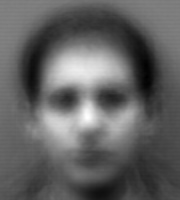
\includegraphics[width=0.3\textwidth]{meanFace.png}
\caption{Mean face of University of Essex male data}
\label{facialRecognition:meanFace}
\end{figure}

\begin{figure}
\begin{subfigure}[b]{0.3\textwidth}
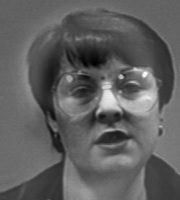
\includegraphics[width=\textwidth]{differenceFace0.png}
\end{subfigure}
\begin{subfigure}[b]{0.3\textwidth}
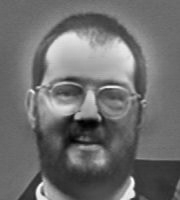
\includegraphics[width=\textwidth]{differenceFace1.png}
\end{subfigure}
\begin{subfigure}[b]{0.3\textwidth}
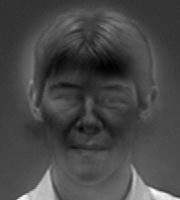
\includegraphics[width=\textwidth]{differenceFace2.png}
\end{subfigure}
\caption{First three difference faces of University of Essex male data}
\label{facialRecognition:differenceFaces}
\end{figure}

\section*{Computing the Eigenfaces with SVD}

With these pelimanaries ready, we are now able to construct the Eigenfaces of the system from the covariance matrix.
At this point we have each image descibed in a vector space with as many pixels as there are in each image.
With the database we are using, this is a 36000 dimensional vector space.
There are too many random variables to work with at this point to work with, so we need to find some way to simplify the vector space.

We do this using the eigenvectors of the covariance matrix (which we call the eigenfaces).
The eigenfaces form a basis of all possible faces, so all faces could be expressed as a linear combination of eigenfaces from the covariance matrix gathered from faces in the database.
The corresponding eigenvalues of the eigenfaces give the weight or importance of each eigenface.
Now there the covariance matrix is still very large 36000 and could have many distinct eigenvectors.
However, only eigenfaces corresponding to higher eigenvalues really make a difference.
Infact, it turns out that there are only as many eigenvalues as there are images in the database.

Recall that taking the SVD of a real valued matrix $A$ gives us the eigenvectors of the matrix $AA^T$ in the columns of $V$.
If the difference vectors are denoted by $E$, then the covariance matrix is $C = EE^T$.
It then follows that we can use the SVD of $E$ to compute the eigenvectors of $C = EE^T$.

The \li{svd} function from \li{scipy.linalg} returns $U,V,V^T$. You can then get the eigenfaces with a call like
\begin{lstlisting}
u,s,vT = la.svd(self.differenceVectors,full_matricies=False)
self.eigenfaces = vT
\end{lstlisting}
This will put into \li{eigenfaces} the eigenfaces of the database as its rows.

\begin{problem}
Implement the function \li{initEigenfaces} by computing the eigenfaces of the images in the database using the SVD and storing them in \li{self.eigenfaces}.
The eigenfaces should be in the columns of \li{self.eigenfaces} so that it becomes a $36000 \times 75$ matrix.
Plot the first three eigenfaces.
\end{problem}

\begin{figure}
\begin{subfigure}[b]{0.3\textwidth}
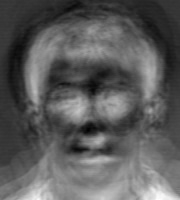
\includegraphics[width=\textwidth]{eigenface0.png}
\end{subfigure}
\begin{subfigure}[b]{0.3\textwidth}
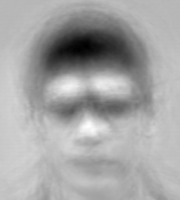
\includegraphics[width=\textwidth]{eigenface1.png}
\end{subfigure}
\begin{subfigure}[b]{0.3\textwidth}
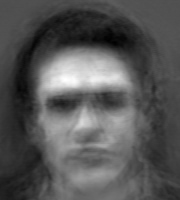
\includegraphics[width=\textwidth]{eigenface2.png}
\end{subfigure}
\caption{First three eigenfaces of University of Essex male data}
\label{facialRecognition:eigenfaces}
\end{figure}

With the eigenfaces computed, we can now convert vectors representing faces into the eigenface space and back.
To convert to the eigenface space we first subtract off the mean face, flatten the vector, then project the vector on the eigenfaces.
To rebuild an image from its representation in eigenfaces, we simply add up the linear combination of eigenfaces then add back in the mean.

\begin{problem}
Implement the functions \li{projectToImageFaceSpace} and \li{rebuildFromEigenfaces}.
\li{projectToImageFaceSpace} should project an image into its coordinates in the basis of the eigenfaces.
\li{rebuildFromEigenfaces} should undo that projection by taking the coordinates in the eigenface space, projecting them back, and reshaping the image.
\end{problem}

\begin{figure}
\begin{subfigure}[b]{0.3\textwidth}
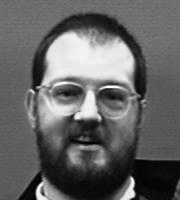
\includegraphics[width=\textwidth]{rebuiltAll.png}
\caption{All the eigenfaces}
\end{subfigure}
\begin{subfigure}[b]{0.3\textwidth}
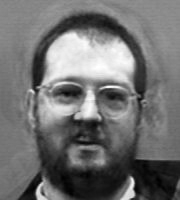
\includegraphics[width=\textwidth]{rebuiltHalf.png}
\caption{Half of the eigenfaces}
\end{subfigure}
\begin{subfigure}[b]{0.3\textwidth}
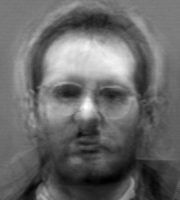
\includegraphics[width=\textwidth]{rebuiltFourth.png}
\caption{Fourth of the eigenfaces}
\end{subfigure}
\caption{Image rebuilt with varying number of eigenfaces}
\label{facialRecognition:rebuiltImage}
\end{figure}

\section*{Creating the Facial Recognition System}

The facial recognition database is almost done. 
Given a face to seach for, we only have to project it into the eigenface basis and then perform a nearest neighbor seach for the closest image.

\begin{problem}
Implement the functions \li{initClassifier}, and \li{findNearest}.
\li{initClassifier} should initialize \li{self.nbrs} as a \li{sklearn.neighbors.KNearestNeighbors} with \li{nearest_neighbors=1}.
Create a set of training points from the images in the database projected into the eigenface basis and use the first \li{searchOrder} number of coefficeints in the \li{self.nbrs.fit} function.
For the labels give the indicies of the labels in the database (this can be done with \li{range})

Implement \li{findNearest} by subtracting off the mean face from the image and then projecting it into the eigenface basis.
Then perform a nearest neighbor search with the coefficeints up to \li{searchOrder} using \li{self.nbrs.predict}.
This will return an index to the matching image.

We also want to compute the distance of the image to the matching image to see if it's really a good match.
Do this by projecting the matching image to the eigenface basis and then taking the norm of its difference from the image passed in but in the eigenface basis.
\end{problem}

\begin{problem}
Verification

Your facial recognition database should be working now.
Try it on some exact images that are in the database, some faces that are in the database but that aren't exact copies, and faces that aren't in the database at all.
(Pick a random image from the full set, it probably won't be in the database. 
 All images that are a multiple of \li{fileStep} are in the database.
 Indicies close to these are probably of the same person but a different picture.
 As you do all of these take note of the distance between the match and the image.
 Chose a reasonable limiting distance to designate a match or false match and add whether this condition is satisfied as a boolean.
\end{problem}